\subsection{Product perspective}

\subsubsection{Scenarios}

    \textbf{Registered users} 
    \vspace{2mm}
    \noindent


    \noindent
    \textbf{User publishes path information in automated mode} 
    \vspace{1mm}
    
    \noindent
    After completing the bike ride,  user U clicks the stop button related to the automated mode and will be redirected to the path data entry page with all the field 
    pre-filled by the system based on the data it collected, with the possibility to modify the status and the obstacles. Finally, U presses the "Publish" button, and the new path becomes immediately visible to all users.

    \vspace{3mm}
    \noindent
    \textbf{User publishes path information in manual mode} 
    \vspace{1mm}
    
    \noindent
    User U wants to share a path they frequently use with the community. From the main map interface, U presses the "Create Path" button (the plus icon). U enters the drawing mode and taps a sequence of points on the map to define the itinerary; the application automatically interprets these inputs and snaps the route line to the correct street geometry. If U is aware of specific obstacles along this route, such as deep potholes or dangerous intersections, U switches the tool to "Obstacles" mode and taps on the corresponding points of the path to flag them. Once the geometry is defined, U proceeds to the next step. The application presents a summary form where U enters the estimated duration and selects a status rating. The system automatically lists the names of the streets detected along the drawn path. Finally, U presses the "Publish" button, and the new path becomes immediately visible to all users.

    \vspace{3mm}
    \noindent
    \textbf{User eliminates a published path} 
    \vspace{1mm}
    
    \noindent
    User U wants to delete a previously published route. In the navbar, U clicks on “Published,” where he will find all the paths they have published. U clicks on the route they want to delete; the page for editing the route’s information will open, and they click on the icon associated with deleting the route.

    
    \vspace{3mm}
    \noindent
    \textbf{User edits the published path}
    \vspace{1mm}
    
    \noindent
    User U views their list of shared routes in the "Published" section and decides to update the details of a specific path due to changed road conditions. U taps on the path card to open the detailed view. To make changes, U presses the "Edit" button (the pencil icon) located in the header. The interface transitions to editing mode: the Start and End location names become editable text fields, and the read-only status badge is replaced by a selection grid, allowing U to quickly switch the rating (e.g., from "Maintenance Required" back to "Optimal"). Additionally, the description field becomes an active text area, allowing U to refine the route notes. Once the modifications are complete, U presses the "Save" button. The application updates the record and immediately reverts to the read-only detailed view, displaying the refreshed information.

    \vspace{3mm}
    \noindent
    \textbf{User modifies personal information}
    \vspace{1mm}
    
    \noindent
    User U wants to edit their personal information. In the navbar, U clicks on “Profile” and then on “Settings”, where he will find all their personal information with the option to modify it

    \newpage
    \noindent
    \textbf{User logs into the application}
    \vspace{1mm}
    
    \noindent
    User U, currently viewing the Home Page in the unregistered state, clicks on "My Profile" in the navbar. This action directs them to the Login screen. On this screen, U is prompted to enter their credentials: they fill in the email address in the designated field and the corresponding password in the password field. After ensuring the data is correct, U clicks on the "Login" button. Upon successful validation, the system grants U access and redirects them back to the main application Home Page, now displaying features and content available to a registered user.
    

    \vspace{3mm}
    \noindent
    \textbf{User discards the collected path information}
    \vspace{1mm}
    
    \noindent
    User U wants to discard the path information he entered. On the data entry screen for the given route, U clicks the “Discard” button, and the information will not be published to the community. However, if the information was entered in automated mode, it will still be added to the recent trips.

    \vspace{3mm}
    \noindent
    \textbf{User saves the trip}
    \vspace{1mm}
    
    \noindent
    User U wants to save the completed trip. Once the trip is finished, the end-of-path screen appears, showing the distance traveled and the average speed, along with the option to submit a report on the path’s status and obstacles. Finally, U clicks the "Back to Dashboard" button and the trips is saved into Recent Trips.


    \vspace{3mm}
    \noindent
    \textbf{User inserts an already existing path}
    \vspace{1mm}
    
    \noindent
    User u enters the information for a new path, but the streets in the entered route are the same as those of an existing path. In this case, the application will notify the user with a warning that the entered streets correspond to those of an already existing path. The same thing happens whether the insertion is done manually or automatically

    \vspace{3mm}

    \noindent
    \textbf{Unregistered users} 
    \vspace{2mm}
    
    \noindent
    \textbf{User registers in the application}
    \vspace{1mm}
    
    \noindent
    User U, having navigated to the Login screen and clicks the "Registration" link presented on this page, is immediately redirected to the dedicated registration page. Here, U is required to complete the registration form by filling in all the necessary information: they enter a valid email address and define a secure password. After reviewing the entered data, U presses the final "Register" button. A verification email will then be sent to the provided email address, containing a verification code that has to be inserted in the application in the appropriate textbox, to confirm that the entered email address exists. Upon successful completion of the registration process, the system confirms the creation of the new account and redirects U back to the main Login screen, prompting them to perform their first access.

    \vspace{3mm}

    \noindent
    \textbf{All users} 
    \vspace{2mm}
  
    \noindent
    \textbf{User searches for a path} 
    \vspace{1mm}
    
    \noindent
     User U wants to find the best path to their destination. From the main map interface, U enters the desired origin and destination points into the floating search bar. The system calculates and displays the five highest-scoring paths on the map. Each path is shown with its associated score, including the visualization of the corresponding obstacles present along the path. The path with the highest score is highlighted in teal to indicate the recommended route, while the other alternatives are displayed for comparison, allowing U to choose the best option before starting the ride.

     \vspace{2mm}
  
    \noindent
    \textbf{User starts a navigation} 
    \vspace{1mm}
    
    \noindent
     After entering the origin and destination and selecting the desired path, user U wants to start navigation.
    From the main map interface, U clicks the "Start Navigation" button, and the navigation screen opens. On the map, a cursor representing U’s current position is displayed; at the top, the current speed and street name are shown, while at the bottom there is an "Exit Navigation" button to end the navigation.

\newpage
\subsubsection{Domain Class Diagram}
    \begin{figure}[!h]
        \centering
        \includegraphics[width=1.1\linewidth]{RASD/Images/Domain Class Diagram.png}
        \label{fig:placeholder}
    \end{figure}

    \noindent
    Notes:
    \begin{itemize}
    \item The \textit{creates} relationship indicates the publication of the Path, while \textit{reports} tracks the contributions regarding obstacles and status, which is then aggregated by the \textit{System} (Merging).
    \item The \textit{status} attribute in \textit{Path} is initially set by the user who published the path, and is later derived from the aggregation of the most recent \textit{PathReport}.
    \item The \textit{structures} attribute in \textit{Path} is a list of points in the map that allows the \textit{System} to draw the path. In manual mode they are manually inserted on the map by the user who publishes the path, while in automated mode they are automatically inserted by the \textit{System}.
    \end{itemize}

\newpage
\subsubsection{State Diagram}
    \noindent
    \textbf{Trip lifecycle} 
    \vspace{2mm}
    \begin{figure}[!h]
        \centering
        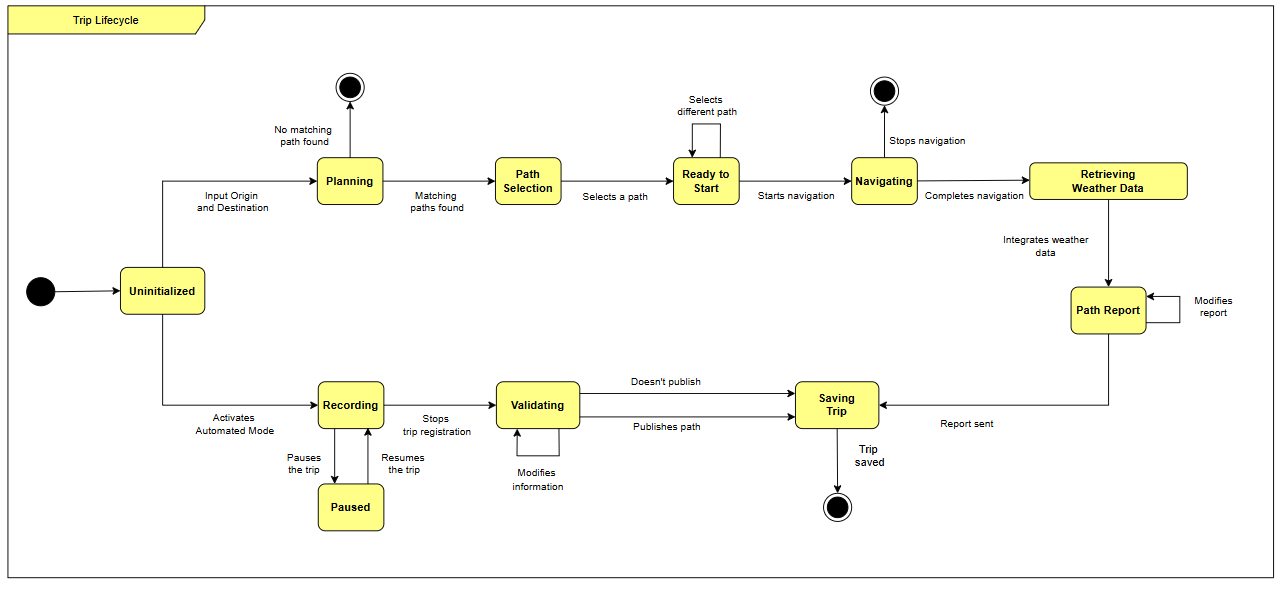
\includegraphics[width=1\linewidth]{RASD/Images/SD_trip_lifecycle.png}
        \label{fig:placeholder}
    \end{figure}
\noindent \\
The Trip lifecycle state diagram illustrates the two operational modes through which the entity is managed by the system.In the upper branch, dedicated to assisted navigation, the user enters the desired origin and destination; the system identifies a set of paths with the highest scores, from which the user selects their preferred route. Navigation is then initiated: during this phase, the system guides the user to the destination while simultaneously recording driving performance metrics. The flow concludes with a review phase, during which data can still be modified before completion.In parallel, the lower branch describes the automated mode, designed for passive tracking: here, the trip immediately enters the recording phase, allowing for intermediate pauses. The recording must then be stopped to proceed to the final validation of the acquired data.Both flows finally converge in the concluding saving state, ensuring that, regardless of the input mode, all metrics, coordinates, and reports are correctly persisted in the system database.
    \newpage
    \vspace{2mm}
    \noindent
    \textbf{Path lifecycle} 
    \vspace{2mm}
    \begin{figure}[!h]
        \centering
        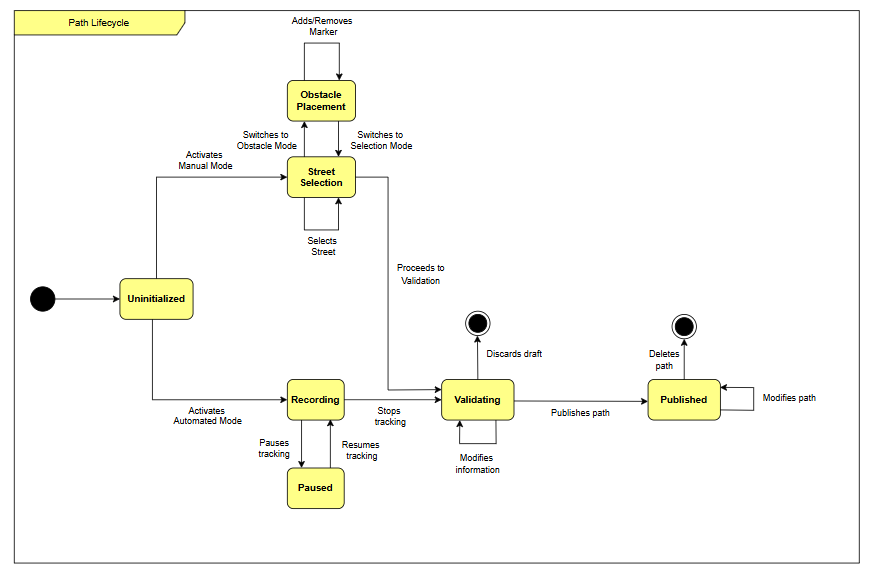
\includegraphics[width=1\linewidth]{RASD/Images/SD_path_lifecycle.png}
        \label{fig:placeholder}
    \end{figure}

\noindent
The Path lifecycle state diagram illustrates the process of creating and publishing a new path within the system. Starting from the initial state, the flow branches into two distinct operational modes.The manual mode allows the user to compose the path by interactively selecting existing streets of interest on the map and manually placing obstacle markers, with the ability to freely switch between these activities.Alternatively, the automated mode acquires the track via real-time GPS recording, handling temporary interruptions through the pause state.Both flows converge in the validation phase; in this state, the user can review and eventually modify the collected information before final confirmation. The cycle concludes with the publication of the path, or with the discard of the draft if not confirmed.

\newpage
    \vspace{2mm}
    \noindent
        \textbf{User Profile lifecycle} 
    \vspace{2mm}
    \begin{figure}[!h]
        \centering
        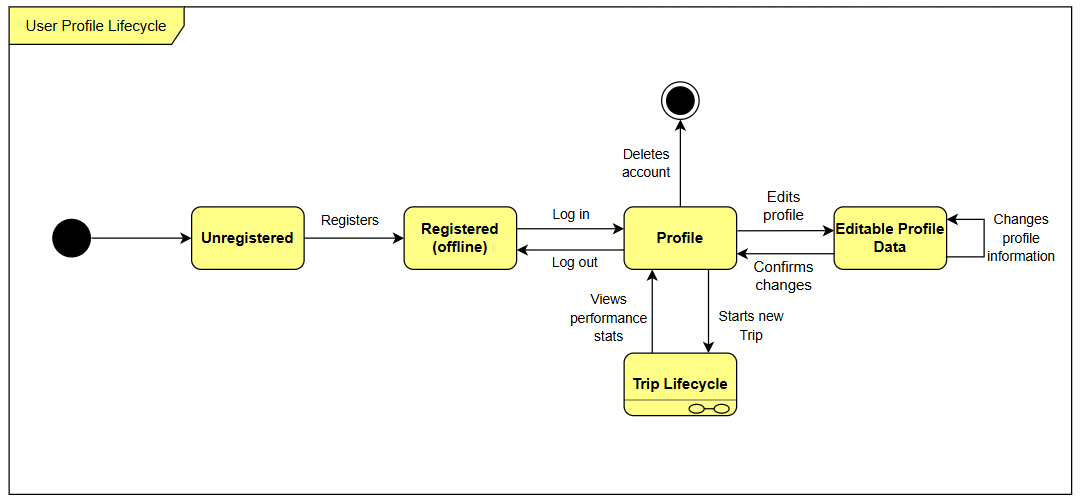
\includegraphics[width=1\linewidth]{RASD/Images/SD_user_profile_lifecycle.png}
        \label{fig:placeholder}
    \end{figure}

\noindent
The lifecycle begins when a visitor without an account completes registration, creating a persistent profile in the system that starts in a signed-out state. Entering credentials activates the working session, allowing the user to modify personal data or undertake new trips to improve their performance statistics. Upon finishing these activities, logging out returns the user to an inactive state while keeping the updated data saved for future access. The cycle ends permanently only if the user chooses to delete their account, an action that irreversibly removes the profile from the system.


\subsection{Product funtions}
    \noindent
    This section outlines the principal functionalities of the platform.

    \vspace{2mm}
    \noindent
    \textbf{Sign up \& Login} 
    \vspace{1mm}
    
    \noindent
     To sign up for the system, a user must provide his name, an email address, and a password. The system checks whether there is an existing account with the same email address: if so, the user is notified that the account already exists; otherwise, the registration proceeds and a verification code is sent to the provided email address. To complete the registration, the user must enter the verification code in the designated textbox.
     To log in, a user must enter the email and the associated password, and the system checks if the credentials match with an existing account: if so, the log in is completed; otherwise, the user is notified that the credentials are wrong.

    \vspace{2mm}
    \noindent
    \textbf{Path search and visualization} 
    \vspace{1mm}
    
    \noindent
     The system allows users to find the best paths that connect two locations. They must enter the starting point and destination, and the system will display on the map the paths with the highest score, along with their related obstacles. It is also possible to access the information screen of the selected path.

    \vspace{2mm}
    \noindent
    \textbf{Publication of a path in manual mode} 
    \vspace{1mm}
    
    \noindent
     The system allows registered users to publish new paths by manually providing the required information.
    The user draws the path and adds obstacles directly on the map, and then enters the remaining information.

    \vspace{2mm}
    \noindent
    \textbf{Publication of a path in automated mode} 
    \vspace{1mm}
    
    \noindent
     The system allows registered users to publish new paths by providing the required information automatically.
    The system retrieves data from GPS and sensors (accelerometer, gyroscope) while the user is biking, and automatically fills in all the necessary information, and the user can choose to accept, modify, or discard it.

    \vspace{2mm}
    \noindent
    \textbf{Navigation} 
    \vspace{1mm}
    
    \noindent
     After the user has selected the desired path from the map and starts navigation, the system provides a real-time representation of the user’s position on the map and also displays the current speed and the street being traveled.

    \vspace{2mm}
    \noindent
    \textbf{Trip tracking and analysis} 
    \vspace{1mm}
    
    \noindent
    The system allows registered users to keep track of their trips. After completing the trip, a screen will appear showing the trip statistics, and once the confirmation button is clicked, the system saves the trip and, if available, enriches it with meteorological information (weather, wind, temperature) retrieved from an external service.

    \vspace{2mm}
    \noindent
    \textbf{Path reporting} 
    \vspace{1mm}
    
    \noindent
    The system allows registered users to submit a report regarding the status and the presence of obstacles on an existing path.
    After completing a trip associated with the path in question, the user can modify the status and add or remove any obstacles, and once the confirmation button is clicked, the report will be sent to the system.

    \vspace{2mm}
    \noindent
    \textbf{Data Aggregation and Merging} 
    \vspace{1mm}
    
    \noindent
    The system collects path reports from multiple users and merges conflicting information. It calculates the current status of a path based on the freshness of the reports and the number of confirming data obtained.

\subsection{User characteristics}

    \subsubsection{Registered users}
    \noindent
    Registered users are able to login to the platform. Their profiles contain personal information and some statistics such as total kilometers travelled, total trips completed, total paths published and the average speed of their trips. In addition to all the features available to unregistered users, they can publish new paths (in either manual or automated mode) and submit reports regarding existing paths. Furthermore, they can record their trips to populate their history and view detailed statistics at the end of the navigation.

    \subsubsection{Unregistered users}
    \noindent
    Unregistered users include casual users, tourists, or people who simply want to find a bike path without tracking their data. They can search for the best paths between two locations, select a desired path, and start the real-time navigation to follow the path, but without the ability to save the trip or view post-activity statistics.

\newpage
\subsection{Assumptions, dependencies and constraints}

    \subsubsection{Domain Assumptions}
    \noindent
    This section describes the fundamental assumptions regarding the environment and the behavior of all entities interacting with the system. These assumptions simplify the system’s design and implementation by setting clear expectations for the users, and the platform itself, ensuring the system functions efficiently within its intended contex

    \begin{description}
        \item[\textbf{[D1]}] The user’s device is equipped with a GPS, an accelerometer and a gyroscope.
        \item[\textbf{[D2]}] The user has a working internet connection.
        \item[\textbf{[D3]}] The user provides truthful information regarding the path to be published.
        \item[\textbf{[D4]}] The user provides truthful reports regarding paths.
        \item[\textbf{[D5]}] The external weather information service is reliable.
        \item[\textbf{[D6]}] The external map service is available and provides accurate topographical data.
    \end{description}

    \subsubsection{Dependencies}
    \noindent
    \begin{itemize}
    \item \textbf{Map Service}: it's responsible for providing the map that enables the graphical visualization of the paths. This is a critical dependency: if this service is unavailable, the core functionalities of the system cannot be performed.
    \item \textbf{Weather Service}: it's responsible for adding weather information to the users’ trips. This is a non-critical dependency: if this service is unavailable, the system will continue to function normally, simply omitting the weather information from the trip details. 
    \end{itemize}